\chapter{Simulation Results \& Discussion}
\label{chap:results}

We perform a large simulation that considers the scattering of small bodies through the Solar System and produce a population of comets that impact Earth. From this we hope to understand how comets, in particular those from the Oort cloud, are injected into the planetary region and onto Earth-crossing orbits. By analysing a range of orbital behaviours exhibited by these comets, we hope to discover interesting and potentially exploitable behaviour in the sky-plane distribution in the months leading up to a comet impact with our planet.

Throughout this analysis we describe `particles' in simulation, with the direction of time going backwards from the point of Earth impact at $t=0$ Myr. Where there is reference of comets, the direction of time is reversed, from a comet's early dynamical lifetime towards an impending Earth impact.

\section{Migration from Earth-crossing orbits}

Reflective of the extreme velocities of LPCs, the majority of particles in the simulation ($\sim60$\%) were immediately ejected onto hyperbolic orbits, and managed to leave the Solar System without becoming captured due to any planetary perturbations. As detailed in \S~\ref{method:evol}, our primary focus in this analysis concerns dynamically evolved comets and their migration through the Solar System.

Fig.~\ref{fig:migration} shows particles that were initially gravitationally bound to the Solar System and that remain bound throughout the length of the simulation. At $t=0$ Myr, all the particles are within the region bounded by the left and right dashed lines, denoting the Earth's aphelion $r_{ap}$ and perihelion $r_{per}$. The left and right dashed lines are described using the equations $r_{ap} = (1+e)a$ and $r_{per} = (1-e)a$. This region is known as Earth's loss cone, and is discussed in more detail in \S~\ref{sec:loss_cone}. 

A common dynamical pathway for many particles in the early stages of the simulation involves particles migrating out of the loss cone because of increases to their semi-major axis, causing them to typically adopt orbits characteristic of NEOs. The majority of these particles then eventually depart the NEO regions after some time and normally adopt orbits around the giant planets, or are ejected. After $\sim2$ Myr the distribution of particles remains roughly constant throughout the Solar System.

Particles with low semi-major axes populate the near-Earth region with aphelia close to that of Earth's. These particles tend to migrate away from Earth with decreasing $a$ up to a point, where they either are rapidly scattered towards regions of the outer Solar System or are returned to orbits close to the Earth-Moon system. It would be reasonable to assume that particles ejected in this manner, that also have low inclination orbits, are likely to collide with the Earth-Moon system again at some point after ejection. As planetary collisions have been neglected in this simulation, it is presumed that the prevalence of such comets remaining close to this region of $a$-$e$-$i$ space in Fig.~\ref{fig:migration} for the majority of their dynamical lifetimes are not realistic.

Particles with eccentricities very close to 1 (as seen located near the horizontal cut-off at the top of the plots) require little energy to become unbound. As expected, these highly eccentric particles rapidly depopulate this area of $a$-$e$-$i$ space within the first few thousand years.

A few particles that are initially ejected onto extreme orbits (very high inclinations $i > 150^\degree$ and high eccentricities $e>0.5$), which have significantly low values of $T_J$ in comparison to the rest of the cometary ejecta, are seen to remain largely undisturbed by planetary interactions throughout the course of the simulation.  Highly inclined orbits minimise time spent close to the ecliptic, reducing the chance of an interaction. These particle retain $a \approx 1$ throughout the 10 Myr length of the simulation.

If one assumes that a LPC has an equal probability to become gravitationally scattered on to any of the available orbital parameters, it is likely that the comet is scattered onto a value of $T_J$ close to its original value (due to the quasi-constant nature discussed in \S~\ref{sec:taxonomy}). Therefore, the probability of LPCs evolving from the Oort Cloud onto extreme orbits with $a$ on the order of Earth's is anticipated to be low. Such particles are expected to have small orbital periods, and remain near Earth for substantially long periods of time - for many orders of magnitude of time longer than their physical lifetimes may permit in this inner Solar System environment.

%FINISH THIS, THEN LOSS CONE (AND PROPER PLOT). Finish discussion with leading onto decision tree. Work out bad comets.
%add a table for something

%finish loss cone and resonance
%find bad comets for plot and mitigation

\begin{figure}[t!]
    \centering
    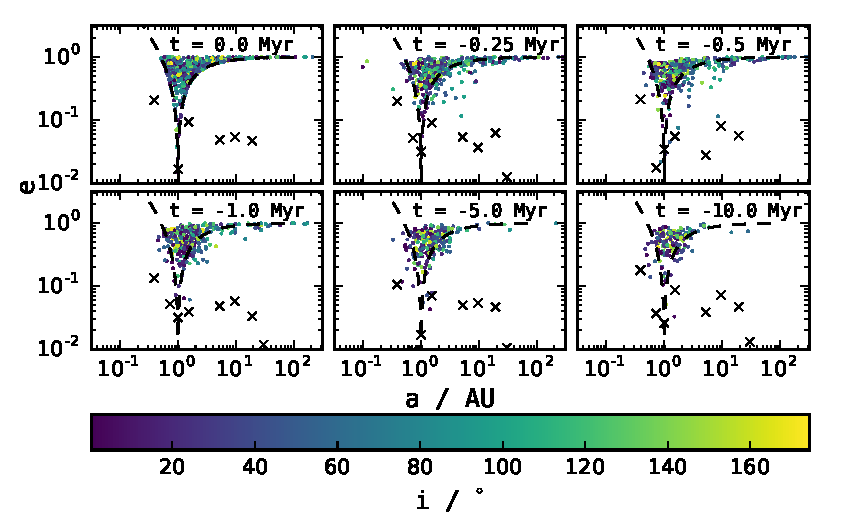
\includegraphics{ae_migration.pdf}
    \caption[Particle Migration]{Gravitationally bound particles in the simulation at various snapshots in time. The boundaries of the Earth's loss cone are marked with dashed lines. The first 8 planets of the Solar System are plotted as black crosses.}
    \label{fig:migration}
\end{figure}

\section{Dynamical lifetimes}

\subsection{Exiting the Solar System}

For each cometary particle in the simulation we calculated the dynamical lifetimes by determining the length of time taken for gravitational perturbations to render the particle's orbit unbound. The median dynamical lifetime was found to be $4.1\times10^5$ yrs. This is of the same order of magnitude as $6\times10^5$ yrs for LPCs reported by \cite{1979IAUS...81..277W}, with a smaller value perhaps indicative of the reduced likelihood for LPCs to reach further into the Solar System and encounter Earth.

The initial population of test particles was observed to decay approximately exponentially for the first 2 Myr of the simulation, before declining at an almost constant rate at times greater than the typical dynamical lifetime. The constant decline in the cometary population at later times is unexpected, as one would assume that the probability of gravitational perturbations by the planets remains unchanged. With a dwindling population of bound particles in the simulation as time progresses, one would expect the leaving rate to continuously decline and the numbers of surviving particles remaining in the simulation to become governed by some form of power law behaviour \citep{1996ASPC..107..233D}. 

We instead find a long-lasting population of comets with dynamical lifetimes exceeding the 10 Myr of the simulation. A subset of this long-lasting population had $a < 2$ AU, and were assumed to be unrealistic due to physical losses due to small heliocentric distances over a long period of time. The remaining objects tended to migrate from the very far reaches of the Solar System ($>$ 600 AU) prior to an impact with Earth. and were found to effectively have become stored in large, stable orbits for periods of time much longer than 10 Myr. 

\subsection{Prograde vs Retrograde orbits}

While the overwhelming majority of asteroids have prograde orbits - many comets (eg. 1P/Halley) are known to have a retrograde orbits. Around 50\% of comets arriving from the Oort Cloud are retrograde.

The energy kicks delivered by the prograde planets upon passing comets should be smaller on average for comets on retrograde orbits than prograde orbits. The result of this is that retrograde comets should have dynamical lifetimes three times longer on average. In the absence of physical decay mechanisms, this means the ratio of retrograde to prograde comets should be 3:1.% This behaviour should manifest itself through the appearance of various transfer pathways for simulated test parts, depending on whether they are prograde or retrograde. 

The initially bound retrograde comets in the simulation had a median dynamical lifetime of $6.4\times10^5$ yrs compared to a median dynamical lifetime of $1.8\times10^5$ yrs for initially bound prograde comets, meaning that the ratio of retrograde to prograde comets should be roughly 3:1 for our simulation. This indicated that prograde comets are more favourably scattered, and that a greater number of much more energetic, retrograde comets reach Earth's orbit.

%Figure.~@@@@@ PUT STUFF HERE

\section{Random Walks in energy space}

\begin{figure}[t!]
    \centering
    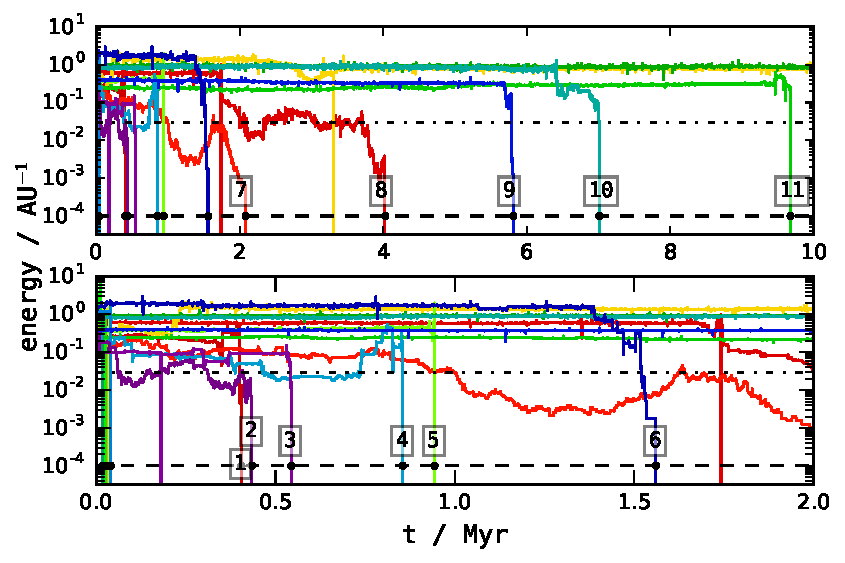
\includegraphics{figures/ae_timeplot.pdf}
    \caption[Random walks in energy space]{Temporal evolution of comet orbital energies. Top: Energy paths of randomly selected comets between $0<t<10$ Myr, shown in different colours. Bottom: Same comets evaluated between $0<t<2$ Myr. Short period comets with P $<$ 200 yr are found above dash-dot black line at 0.0292 AU$^{-1}$.  Comets beginning their dynamical evolution through the Solar System are found below the dashed black line at $10^{-4}$ AU$^{-1}$. Black dots mark the transitions of comets coming from dynamically new regimes for the first time, between the times 0.05-10 Myr, and are labelled for reference.}
    \label{fig:timeplot}
\end{figure}

%http://adsabs.harvard.edu/full/1980A%26A....85...77Y diffusion eq
An analysis of the scattering mechanisms of dynamically new LPCs that are just beginning their evolution through the Solar System is an important first step in considering how comets  either i) migrate towards more tightly bound orbits and deeper into the Sun's gravitational potential towards Earth, or ii) are scattered onto unbound orbits and quickly leave the Solar System.

The dynamical evolution of LPCs through successive interactions with planets in the Solar System is often described as a stochastic process, in which a comet interacts every successive perihelion passage with a planetary configuration unique to the previous interaction. As LPC aphelia lies well beyond the reach of the Solar System, the planets' gravitational influence dominates at perihelion passage, and can be approximated with an instantaneous kick in orbital energy, where $x = (1/a)$ is the binding orbital energy of an object on a Keplerian orbit. These kicks are symmetrically distributed about zero, and are uncorrelated as long as the comet's orbital period remains much larger to that of the planets. 

The energy of highly eccentric comets evolves on much shorter time scales than orbital elements such as perihelion $q$, inclination $i$, longitude of ascending node $\Omega$, argument of perihelion $\omega$. Therefore one can, as a first-order approximation, conceive the orbital evolution of LPCs as a one dimensional random walk behaviour in energy space. This is distinct from other more dynamically evolved objects in the Solar System which exhibit different dynamics, (eg. those with resonant behaviours). 

This behaviour is exhibited in Fig.~\ref{fig:timeplot} where we can observe the random walk behaviour of LPCs injected into the planetary system. We consider two absorbing walls in energy space; ejection onto an unbound orbit $(x > 0$ AU$^{-1})$ , and transfer to a periodic regime $(x < 0.0292$ AU$^{-1})$ corresponding to $P < 200$ yr (dot-dashed line). Dynamically young comets, probably on their first passage into the Solar System from the Oort Cloud, have energies below $(x < 10^{-4}$ AU$^{-1})$ (dashed line).

While most comets are rapidly injected towards the periodic orbit energies, some comets persist in energy space between the two absorbing walls for considerably lengths of time. We find an excess of paths in Fig.~\ref{fig:timeplot}, notably 6,7 and 8, that correspond to retrograde comets. This demonstrates that retrograde comets evolve much slower in this energy space due to lower probabilities of being caught by the planets. Such lengths of time spent in the outer reaches of the Solar System suggest that retrograde comets have ample time to fade sufficiently, before progressing to dynamically older states in regions in which they can more easily be observed from Earth.

Prior to an impact with Earth, 3, 4, and 8 in in Fig.~\ref{fig:timeplot} can be seen to have entered the region in energy space between $(0.0292 < x < 10^{-4}$ AU$^{-1})$. Such behaviour is believed to be unlikely as the typical energy change of a comet per revolution is of the order $\sim10^{-3}$ AU$^{-1})$. A return to `dynamically newer' states may also be unrealistic once non-gravitational forces are taken into account. The actions of non-gravitational effects may complicate the simple statistical considerations of randomly-walking comets, and provide systematic increases or decreases to the orbital energy of comets. The result of this means that the dynamical evolution of comets is much faster once non-gravitational considerations are met, leading to comets becoming much less sensitive to transitions to and from this dynamically new region of energy space.

Some comets, for example those following the paths 1, 5, 9, 10 and 11, are rapidly injected into the Solar System, spending no more than a few perihelion passes in the space between the two absorbing walls. These comets quickly find themselves in long-lasting, tightly-bound orbits where the systematic gravitational effects of the planetary environment become much more relevant. The oscillatory behaviour of the orbital energy suggests these comets have quickly become trapped in stable orbits governed by mean motion resonances (MMRs) (see \S~\ref{sec:resonance}).

%https://projecteuclid.org/download/pdf_1/euclid.bsmsp/1200512808

\section{Resonance}
\label{sec:resonance}

Although generated with cometary dynamical properties, some particles throughout the simulation behaved strikingly similar to NEAs, which are known to chaotically migrate from the inner Solar System due to the effects of repeated close encounters with terrestrial planets, and the effects of MMRs and secular resonances.

Once becoming ejected from the Earth-Moon system, some particles in the simulation have scattered between the terrestrial planets before eventually entering stable orbits via strong resonances. These resonances are easily detected from the analysis of the temporal evolution of $a$, identifying where there are small-amplitude oscillations around a constant mean value $\langle a \rangle$. 

We study MMRs in particular by studying the mean averages of $a$ in windows of $10^4$ yrs. We identify the locations of $p$:$q$ resonances using $a_{mmr} = a_p (p/q)^{2/3}$ where $a_p$ is a planet's semi-major axis. This reveals a distribution in $\langle a \rangle$ with strong peaks corresponding to resonances up to the 1:21 external MMR with Jupiter. The majority of comets `stuck' in these stable librations are retrograde, which can be understood by the reduced influence of Jupiter on retrograde orbits. 

We also find peaks in $\langle a \rangle$ revealing large Trojan populations of comets stuck in 1:1 capture resonances with Jupiter and Neptune. For all comets stuck in these MMRs, we found that at least 20\% of their dynamical evolution time was spent within $\pm.1$ AU of any of these resonances. We also find comets become captured into Saturn and Uranus crossing orbits, but find themselves ejected quickly, possibly due to an orbital instability introduced by Jupiter.

Throughout a comet's lifetime both random walk and resonant behaviour become important at separate points in time, as well as largely influential for particular classes of comets. In the simulation, the long-term survival of the particles ended up being much greater than predicted by purely diffusive behaviour - a result attributed to the interplay of both these dynamical behaviours.

From Table.~\ref{table:class}, one can see that the particles that migrated from Earth and into the Centaur dynamical class spent an average of $3/4$ of their dynamical lifetimes with this behaviour. From the population of these Centaur particles we find that migration from Earth-crossing orbits is a rapid and chaotic path through the Solar System, rapidly raising their $a$ up to distances comparable to Uranus' in an amount of time equal to the average of 3\% of their dynamical lifetimes. A qualitative analysis of the Centaur particles revealed two distinct groups - one consisting of comets characterised by diffusive behaviour, and  another group of Centaurs dominated by resonant behaviour for almost the entire lengths of their dynamical lifetimes. Particles were likely to leave the Centaur class by evolving to HFCs or JFCs. There was a clear predominance of retrograde orbits for the particles that exited the Centaur class by rapidly moving towards Oort Cloud energies.

The populations with $q < 1.3$ AU of the HFCs and JFCs in the simulation remained of comparable size throughout the length of the integration. HFCs were likely to become gravitationally ejected after migrating into MMRs with Jupiter, in particular the exterior 1:q exterior resonances. JFCs, being more strongly coupled with Jupiter, were more likely to remain bound and migrate outwards to the far reaches of the Solar System.

\begin{table}[t!]
\centering
\caption[Particles classes and their mean dynamical lifetimes]{Classifications of test particles in the simulation and the average \% of the particle's dynamical lifetime spent in that class. Classifications into either a Jupiter Family Comet (JFC), Halley Family Comet (HFC), Centaur, Trans-Neptunian Object (TNO) or Encke-type comet. Class definitions based on the Jovian Tisserand parameter $T_J$, orbital period $P$, perihelion $q$, and semi-major axis $a$.}\vspace{1.5ex}
\label{table:class}
\begin{tabular}{ccc} \toprule \toprule
Taxonomic Class & Classification                                      & Mean \% dynamical time \\ \midrule
JFC             & $2 < T_J < 3$; $P > 20$ yrs & 26.86                  \\
HFC             & $T_J < 2$; $P < 200$ yrs               & 42.60                  \\
Centaur         & $q > 5.2$ AU, $a < 30.1$ AU          & 69.18                  \\
TNOs            & $a > 30.1$ AU                              & 26.13                  \\
Encke-type          & $T_J > 3$; $a < 5.2$ AU             & 70.31                 
\end{tabular}
\vspace{-3ex}
\end{table}

%leave resonances by increase in libration or A torque is applied that is stronger than the resonance can tolerate.
%https://history.nasa.gov/SP-345/ch8.htm
%MAIN BELT COMETS
%ALSO IN 1:1 WITH NEPTUNE


%more from %https://arxiv.org/pdf/1606.05603.pdf

%stable vs unstable resonances capture resonances
%commensurabilit/near commensurability
%BREAKING THE RESONANCE Comets: Nature, Dynamics, Origin, and their Cosmogonical Relevance resonance P85

%Resonance Hopping vs random walk diffusion LOOK AT THIS
%https://eprints.usq.edu.au/28888/1/CentaursJeremy.pdf

%this study supports the idea that Centaurs do represent a threatto Earth.
%Of thetaxonomicalclasses inward from the resonance, the Encke-type cometclass had the highest average occupancy time at 33\%. Of the outward classes,KBO had the highest average occupancy time at 14.9\% of a test particle’s lifetime. 65\% of a sample of Earth crossers were random walkers and 35\%resonancehoppers.Graphs of semi-major axis vs. time for resonance-hopping Centaurs tend to have long horizontal bands, and those of the random-walk Centaurs tend to lack long horizontal bands

\section{The Encke Problem}

Of the taxonomical classes in Table.~\ref{table:class}, the Encke-type comets made up the longest occupancy times at 70\%. The comets were decoupled from Jupiter, with aphelia $Q < 4.2$ AU, with $a$ interior the Jupiter 3:1 MMR and $a < 2.4$ AU. These comets typically find themselves embedded in asteroid populations at low inclinations; these asteroid populations themselves perhaps consisting of extinct cometary nuclei. Object in these orbits constitute a significant fraction of the Earth impact flux.

Of all the Encke-type comets investigated in the simulation, the second most likely dynamical class for such objects to be in during their lifetimes was found to be the HFC class. This reveals the presence of a purely gravitational dynamical pathway (produced by the terrestrial planets) for LPCs to rapidly evolve into Encke-type classes. This is of particular significance, as it suggests that a large population of dormant comet nuclei may exist in NEO populations, masquerading as asteroids and therefore impacting our understanding  of  the  relative  importance  of  asteroids  compared to comets as part of the impact hazard.

The majority of these comets' lifetimes were found to be spent in this Encke-type class, with a median dynamical lifetime of 7.89 Myr. This suggests that like the asteroids which such comets cohabit regions of the Solar System with, the small body populations are unlikely to fluctuate wildly on short-term, human timescales due to the introduction of a comet shower. Additionally, the dynamical lifetimes far exceed the expected estimated amount of time required for a comet to physically age, and become dormant or fragment. This suggests that redoing the simulation with realistic modelling of the physical aging of comets would apply additional constraints on these Encke-type comets -  and allow only anomalously large and long-lived comets to persist into such orbits. Alternatively, it could also mean that a population of multi-kilometre, long-lived and extreme low albedo comets could exist in the NEO environment, unbeknownst to current Earth object surveys.

%encke Type comet impacts
%comet fading to dormant JFCs
%https://pdfs.semanticscholar.org/db45/cffd0d3ef903498c5e80b2358d3f632717a7.pdf
%we define ‘Encke-like’to mean those objects decoupled from  Jupiter (Q<4.2AU)with semi-major axes interior to Jupiter’s 3:1 mean motion reso-nance (a<2.4 AU). 

%size and shapes of cometary nuclei http://adsabs.harvard.edu/abs/2004come.book..223L
%http://www.astro.uwo.ca/~wiegert/papers/2006Icarus.182.161.pdf
%\section{Fragmentation}

%clustering of aphelion directions
%exotic particles
%random walk and resonance hopping
%\cite{1997astro.ph..5153W}

\section{Jupiter-Saturn Barrier}
\label{js-barrier}
%https://arxiv.org/pdf/0911.4381.pdf
As infalling comets proceed on a random walk in $1/a$, the planetary energy kick imparted by the giant planets in the 10-15 AU range is typically much larger than the gravitational binding energy of inbound Oort Cloud comets that are only tenuously bound to the Solar System. Therefore, the expected perihelion drift of LPCs falling into the inner Solar System is expected to halt in the $\sim$10-15 AU domain where comets become rapidly unbound from the Solar System, or perturbed onto low $a$ orbits before then eventually becoming ejected. This mechanism, known as the Jupiter-Saturn barrier, is hugely influential in influencing cometary motion, responsible for significantly reducing the impactor population reaching Earth.

Analysis of all the Earth impactors that pass through the Jupiter-Saturn zone revealed that a smooth drift in $q$ followed by a rapid inflation in $a$ that occurs around the 15 AU point - as LPCs move inwards toward regimes of more rapid orbital evolution. This effect obscures the Oort Cloud origin of such comets, but more importantly allows them to prevail against the `leaky' Jupiter-Saturn barrier. 

Retrograde comets are again observed to be more successful in penetrating the barrier, due to weaker planetary perturbations.

Objects with $a\sim 3\times10^4$ were particularly efficient in circumventing ejection by the Jupiter-Saturn barrier - partly because these objects would require less energy kicks by the planets to reach perihelion distances beyond the gas giants. No particles in the simulation were found to move through the Jupiter-Saturn barrier with diffusive behaviour characterised by a nearly constant $a$ - the orbital evolution of the particles was instead markedly dominated by rapid changes in $a$. When analysing the distribution of $\langle q \rangle$, the moving average of perihelia in windows of $10^2$ yrs, no particles were found to have $10 < \langle q \rangle < 20$ AU.

Many particles in the simulation that persisted safely throughout the inner Solar System then became ejected upon reaching the Jupiter-Saturn zone in their backwards integrations. This suggests that Jupiter and Saturn provide a very efficient barrier effect that places large constraints on the various dynamical pathways towards the inner Solar System through the 10-15 AU range. These ejected particles represent comets that may not have realistically overcome the Jupiter-Saturn barrier when evolving forwards in time.

The larger the value of $a$, the less of a perturbation comets encounter from the Jupiter-Saturn barrier. Therefore, inbound LPCs that have been thrown out of the Oort Cloud by a strong perturber such as a close passing star are more likely to overcome the barrier as opposed to comets with smaller $a$, due to perhaps being perturbed by the galactic tide. This raises the prospect of an exceptionally large comet shower overcoming the barrier over short timescales. The ensemble of orbits in a comet shower passing the Jupiter-Saturn zone all at once would manifest itself as the rapid population of a somewhat sparse region of velocity space known as the loss cone (detailed in \S~\ref{sec:loss_cone}). %TALK ABOUT COMETS SHOWERS and leads into jupiter/loss cone segue
%Objects in a comet shower from the Oort Cloud are likely to have velocity vectors close to the solar direction, part of the configuration of a comet's orbit that makes it liable to removal through a range of dynamical and physical processes due to interaction with the Sun.
%p7 https://arxiv.org/pdf/1801.01474.pdf

\section{Loss Cone Dynamics}
\label{sec:loss_cone}

\begin{figure}[t!]
    \centering
    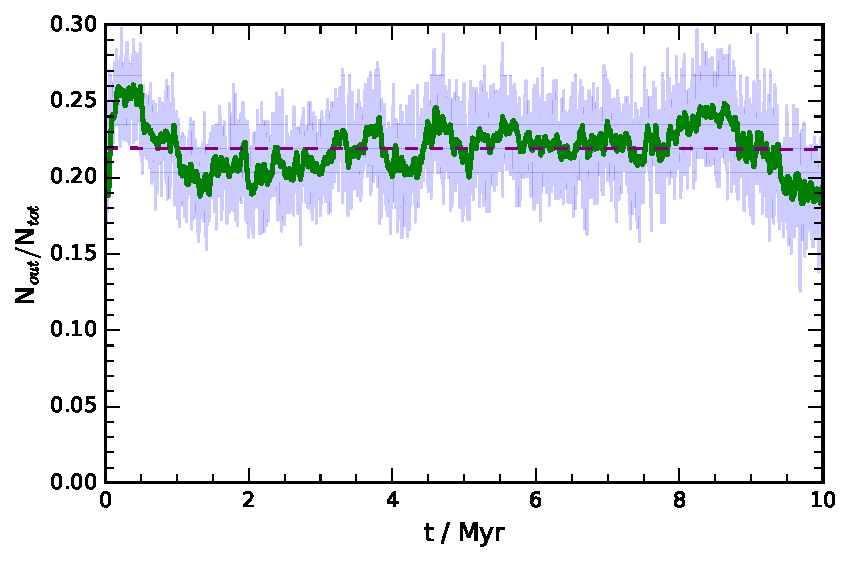
\includegraphics{figures/exotic_ratio.pdf}
    \caption[]{}
    \label{fig:exotic}
\end{figure}

A population of comets falling inwards from the Oort Cloud will have randomly oriented orbits where all approach directions are possible. Comets falling very close the solar direction are likely to get boiled away and disintegrated by the Sun, or alternatively may swing by one of the planets and pick up enough extra speed from the encounter to carry it right out of the solar system. In either case, these particular comets are lost from the Solar System. Consequently, there is an region of energy-angular momentum space around the solar direction that is expected to be particularly devoid of LPCs. This is known as the Sun's loss cone, and was shown by \cite{1981AJ.....86.1730H} to be effective in shielding the Earth from showers of comets.

This loss cone concept is similar to considerations of stars or stellar remnants accreting into black holes \citep{0264-9381-30-24-244005}. The formulation of a loss cone can be extended to other bodies of the Solar System, and is described as a set of orbits of sufficiently low angular momenta such that they intersect a certain body, or pass within some distance of its centre. %The critical angular momentum $J_{lc}$ of a loss cone for a periapsis of the central body $q$ is,

%\begin{equation}
%    J_{lc}^2 = GM_\odot q(1+e)~.
%\end{equation}

%Comets with $J < J_{lc}$ fall within the loss cone and are assumed to become removed over some timescale corresponding to the loss cone's central body.

External perturbations on the Oort Cloud, eg. passing stars, can significantly change the angular momenta of comets and send them into the Sun's loss cone. The Jupiter-Saturn barrier (detailed in \S~\ref{js-barrier}) is unable to provide sufficient orbital angular momenta to such comets for them to leave the loss cone. A loss cone comet can only leave the region by two means; through either hyperbolic ejection, or the destruction of the comet due to breakup near the Sun or a planetary impact. This means that if there is the occurrence of an exceptionally strong shower of Oort Cloud comets, such an event can manifest itself as a rapid filling of the Sun's loss cone, and can therefore be a method of identifying an impending LPC threat to Earth.

In this investigation, we simulate a huge number of comets reaching Earth within an 11.8 year period. Comets capable of an impact with Earth have heliocentric loss cone orbits - which means that the simulation is in effect - an unrealistically very extreme example of a comet shower filling the Sun's loss cone. In addition, we are not concerned in retracing these comets back to an Oort Cloud environment (for reasons detailed in \S~\ref{sec:accuracy}). For these reasons, we neglect analysis of the filling of the Sun's loss cone and focus on smaller regions of angular-momenta space within it, namely the Earth's and other planet's loss cones.
%spend time considering earth loss cone for this sim - we cant really do sun loss cone as we're doing a comet shower anyway
%reference mpc data and talk about how phas are almost all in loss cone of earth

Fig.~\ref{fig:exotic}

\section{Worst-case scenarios}

\begin{figure}[t!]
    \centering
    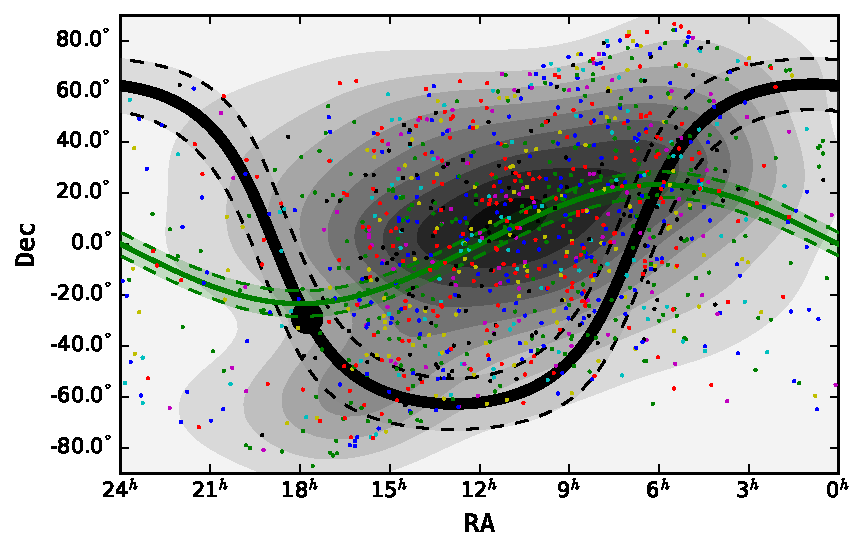
\includegraphics{radiants.pdf}
    \caption[Distribution of apparent radiants]{Distribution of apparent radiants. Geocentric equatorial coordinates plotted for various comet threats. Green line and boundaries represent the plane of the ecliptic $\pm5^\degree$, black line and boundaries represent the galactic plane $\pm10^\degree$. The galactic centre is plotted as black circle. A 2D kernel density estimate is shown.}
    \label{fig:loss_cone}
\end{figure}

% "In principle," he adds, "one would expect those positions to be evenly distributed in the sky, particularly if these objects come from the Oort cloud. However, what we find is very different-a statistically significant accumulation of radiants. The pronounced over-density appears projected in the direction of the constellation of Gemini, which fits the close encounter with Scholz's star.


%prograde vs retrograde plot
%https://onlinelibrary.wiley.com/doi/pdf/10.1111/maps.12080 make fig5
%radiant distribution plot for good lasting comets geocentric equatorial
%lead time calculations
%decision tree of loss cone direct entry time, choose features that match mpc



%dormant comets
%http://adsabs.harvard.edu/full/2004MNRAS.355..191N
%https://academic.oup.com/mnras/article/462/4/3511/2589444





\iffalse

%We operationally define τ stream as the time taken for the median D-parameter of any two test meteoroids to grow beyond a given threshold. The D-parameter was originally introduced by Southworth & Hawkins (1963) for meteor shower identification; it is essentially a measure of the similarity between a pair of orbits denoted as A and B:

\begin{equation}
\begin{split}
    D_{A,B}^2 = (q_B - q_A)^2 + (e_B - e_A)^2 + \left(2\sin{\dfrac{I}{2}}\right)^2
    \\ + \left[(e_A + e_B)\sin{\dfrac{\Pi}{2}}\right]^2 ~,
\end{split}
\end{equation}

where,

\begin{equation}
\begin{split}
    I = \arccos[{\cos{i_A}\cos{i_B}+\sin{i_A}\sin{i_B}\cos{\Omega_A-\Omega_B}}]~,\\
    \Pi = \omega_A - \omega_B + 2\arcsin{\left(\cos{\dfrac{i_A + i_B}{2}\sin{\dfrac{\Omega_A - \Omega_B}{2}\sec{\dfrac{I}{2}}}}{}\right)}~.
\end{split}
\end{equation}

\fi